% Created 2021-05-06 Thu 09:04
% Intended LaTeX compiler: pdflatex
\documentclass[11pt]{article}
\usepackage[utf8]{inputenc}
\usepackage[T1]{fontenc}
\usepackage{graphicx}
\usepackage{grffile}
\usepackage{longtable}
\usepackage{wrapfig}
\usepackage{rotating}
\usepackage[normalem]{ulem}
\usepackage{amsmath}
\usepackage{textcomp}
\usepackage{amssymb}
\usepackage{capt-of}
\usepackage{hyperref}
\usepackage{minted}
\usepackage{tabularx}
\author{Philipp Beer}
\date{2021-05-10}
\title{592 Project Report}
\hypersetup{
 pdfauthor={Philipp Beer},
 pdftitle={592 Project Report},
 pdfkeywords={unic, 501dl, stassopoulou},
 pdfsubject={Literature review in time series clustering},
 pdfcreator={Emacs 27.2 (Org mode 9.4)}, 
 pdflang={English}}
\begin{document}

\maketitle


\section*{Project Report 592 Project in Data Science}
\label{sec:orgb3a03c7}
Philipp Beer
Gradudate Program Data Science at UNIC, Nicosia Cyprus

COMP-501DL Research 
Prof. Spyros Makridakis
Prof. Ioannis Katakis
\subsection*{Introduction}
\label{sec:org7698451}
\subsubsection*{M4 Competition Forecasting}
\label{sec:orgb90c57d}
\subsection*{Approach}
\label{sec:orge68be3e}
\subsection*{Time Series  Properties}
\label{sec:org1095d09}
\subsubsection*{ts fresh}
\label{sec:orgb505caf}
\subsubsection*{Feature Extraction}
\label{sec:orge6e2efd}
\subsection*{Clustering}
\label{sec:org3ffc334}
\subsubsection*{Deciding k}
\label{sec:org3667df5}
\subsection*{Forecasting}
\label{sec:org9d26251}
\subsubsection*{Cross-Validation}
\label{sec:orgf4ef268}
\subsection*{Benchmarking}
\label{sec:orgf1ac54f}
\subsection*{Challenges}
\label{sec:orgbbd4989}
\subsubsection*{Data Preprocessing}
\label{sec:org6e443f2}
\subsubsection*{Computational Costs}
\label{sec:org3b8bf12}

\subsection*{Results}
\label{sec:orgf761d1f}
\subsection*{Conclusion}
\label{sec:org03020af}
\subsubsection*{Results of Cross-Validation}
\label{sec:org1432392}
\begin{center}
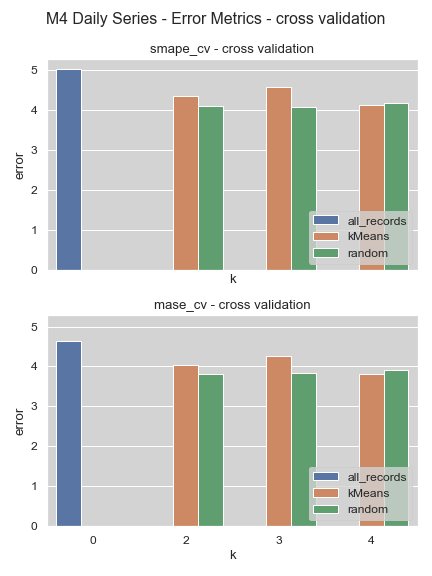
\includegraphics[width=.9\linewidth]{../img/daily_cv_results.png}
\end{center}
\subsubsection*{Results on M4 test set}
\label{sec:orgfeee714}
\begin{center}
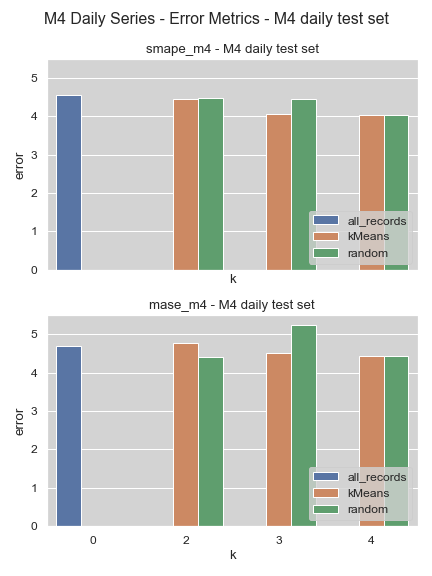
\includegraphics[width=.9\linewidth]{../img/daily_m4_results.png}
\end{center}
\subsubsection*{}
\label{sec:org1c83b2e}
\subsubsection*{results not better than random}
\label{sec:orgc25adc4}
\subsubsection*{Uncertainty in the clustering}
\label{sec:org41c56d2}
\subsubsection*{}
\label{sec:orgd25c4cf}

\subsection*{How to measure similarity}
\label{sec:org54cd60f}
\subsection*{Ts representation}
\label{sec:org9d8aedf}
\subsection*{Distance metrics}
\label{sec:org50d233d}
\subsection*{Clustering algorithms}
\label{sec:org99fb8e8}
\subsection*{Limitations}
\label{sec:orgf00b172}
\subsection*{Conclusions}
\label{sec:org0eba474}

\#\#\#\# this the old template

\section*{Flajolet-Martin Implemenation}
\label{sec:org97e4cf6}
\url{https://552dlimages.s3-eu-west-1.amazonaws.com/unic\_logo.png}

Philipp Beer
\subsection*{Counting cardinalities of Wikipedia entries}
\label{sec:org50d2da2}

University of Nicosia

COMP 552DL - Data Privacy and Ethics

Prof. Dr. Thomas Liebig
\section*{Motivation}
\label{sec:orga68a06d}
\begin{itemize}
\item counting cardinalities with limited resources (Big Data)
\item flow monitoring from stationary sensors
\end{itemize}
\subsection*{Wikipedia Entry Cardinalities}
\label{sec:orgf5d2bd2}
\begin{itemize}
\item Wikipedia large variety of cardinalities across its entries
\item readily available API for data ingestion
\end{itemize}

\section*{Flajolet-Martin Algorithm}
\label{sec:orgaddfa05}
\subsection*{Basic Estimation Approach}
\label{sec:org7773de8}
\subsubsection*{Hash Function}
\label{sec:org8ca99e8}
word is denoted as:
$$ x = (x_0, x_1, \dots, x_p) $$

Elements of x are hashed via:
$$ hash(x) = (M + N \sum\limits_{j = 0}^p ord(x_j) 128^j)\: mod \: 2^L $$
\subsubsection*{Resulting Integer}
\label{sec:org6e7c8db}
is considered in its bit form:
$$  y = \sum_{k \ge 0} bit(y, k)\,2^k $$

where p(y) represents the postion of the least-significant set bit.
\subsubsection*{Bitmap}
\label{sec:org870f388}
$$p(y)$$ for each word in stream is stored in a $$bitmap[0 \ldots L-1]$$
\begin{itemize}
\item Length of Bitmap $$L > log_2(n/nmap) + 4$$
\end{itemize}
\subsubsection*{Expected Behavior}
\label{sec:org269c977}
If n is the number of distinct elements in M then:
\begin{itemize}
\item bitmap[0] is accessed approximately n/2 times
\item bitmap[1] is accessed n/4 times
\item \ldots{}
\end{itemize}
\subsubsection*{In consequence}
\label{sec:org10504cd}
$$ i \gg \log_2\,n $$ is expected to be zero
$$ i \ll \log_2\,n $$ is expected to be one
$$ i \approx log_2\,n$$ has a fringe of zeros and ones
\subsubsection*{Bias Factor}
\label{sec:orge291dad}
Flajolet and Martin identified a bias factor:
$$ \varphi = 0.77351\cdots$$
\subsubsection*{Standard Deviation}
\label{sec:org7be49cc}
Flajolet and Martin prove that under reasonable probablistic assumptions:
$$ \sigma(R) \approx 1.12$$
Therefore, result is typically 1 binary order of magnitude off (correction via nmap)
\subsubsection*{NMAP}
\label{sec:orga26f4cd}
Set of Hashing functions for each word
$$  A = \frac{ R_1 + R_2 + \dots + R_m}m $$


\subsection*{PCSA}
\label{sec:org0713c8f}
Probabilistic Counting with Stochastic Averages
\subsubsection*{Modification to basic approach}
\label{sec:orgd7cab22}
\begin{itemize}
\item use hashing function in order to distribute each word into one of m lots via:
$$ \alpha = h(x)\,mod\,m$$
\item update corresponding bitmap vector of alpha from h(x)
$$ h(x)\: div\: m$$ (floored)
\end{itemize}
\subsubsection*{Expectation}
\label{sec:org292c374}
\begin{itemize}
\item distribution of records falls evenly into lots so that $$(1/\varphi)\,2^A$$ is a reasonable approximation
\end{itemize}
\subsection*{Implementation}
\label{sec:org4001509}
\subsubsection*{Hash Function}
\label{sec:org012b0d4}
\begin{minted}[frame=lines,fontsize=\scriptsize,xleftmargin=\parindent,linenos,breaklines=true]{python}
def hash_val(self, word: str, v: int, w: int) -> int:
       l = list(word)
       term1: int = 0
       for i in range(len(l)):
	   term1 += ord(l[i])*128**i
       return int((v*term1 + w) % 2**self.L)
\end{minted}

\subsubsection*{Updating the bitmap}
\label{sec:org87bea05}
\begin{minted}[frame=lines,fontsize=\scriptsize,xleftmargin=\parindent,linenos,breaklines=true]{python}
def update_bitmap(self, word: str) -> None:
	# calculate hash value
	for i in range(self.nmap):
	    # calculate hash with current set of values
	    hash_val = self.hash_val(word=word,
				     v=self.vs[i],
				     w=self.ws[i])
	    # find rightmost set bit in hash value
	    r = self.rightmost_set_bit(hash_val)
	    if r == None:  # cases need to be ignored as element value is 0
		continue
	    assert type(r) == int, 'r must be int'
	    if self.bitmaps[i, r] == 0:
		self.bitmaps[i, r] = 1
\end{minted}

\subsubsection*{Rightmost Set Bit}
\label{sec:org19349d9}
\begin{minted}[frame=lines,fontsize=\scriptsize,xleftmargin=\parindent,linenos,breaklines=true]{python}
def rightmost_set_bit(self, v: int) -> int:
	# using bit operations to identify position
	# of least significant set bit
	if v == 0:
	    return None
	return int(math.log2(v & (~v + 1)))
\end{minted}

\subsubsection*{Basic Estimation Approach}
\label{sec:org2619bfd}
\begin{minted}[frame=lines,fontsize=\scriptsize,xleftmargin=\parindent,linenos,breaklines=true]{python}
def fm(self) -> int:
	# allowing for hashing of entire stream
	vbitmap_update = np.vectorize(self.update_bitmap)
	# contains hashed values for each element in stream
	vbitmap_update(self.data_stream)

	if self.optimization == 'reduce':
	    # reduce bitmap
	    red_bitmap = self.reduce_bitmaps(self.bitmaps)
	    R = self.leftmost_zero(red_bitmap)
	    return self.C*2**R
	elif self.optimization == 'mean_r':
	    R = np.zeros((self.nmap,))
	    for i in range(self.nmap):
		R[i] = self.leftmost_zero(self.bitmaps[i, :])
	    mean_R = np.mean(R)
	    return self.C*2**mean_R
\end{minted}

\subsubsection*{PCSA Approach}
\label{sec:org0187011}
\begin{minted}[frame=lines,fontsize=\scriptsize,xleftmargin=\parindent,linenos,breaklines=true]{python}
def pcsa_bitmap(self, word: str) -> None:
    hashedx = self.hash_val(word=word,
			    v=self.m,
			    w=self.n)
    alpha = hashedx % self.nmap
    beta = math.floor(hashedx/self.nmap)
    assert isinstance(beta, int), "index is integer"
    idx = self.rightmost_set_bit(beta)
    self.bitmaps[alpha, idx] = 1

def fm_pcsa(self) -> int:
    # allowing for hashing of entire stream
    vbitmap_update = np.vectorize(self.pcsa_bitmap)
    # contains hashed values for each element in stream
    vbitmap_update(self.data_stream)
    S = 0
    for i in range(self.nmap):
	R = 0
	while (self.bitmaps[i, R] == 1) and (R < self.L):
	    R += 1
	S += R
    return math.floor(self.nmap/self.phi*2**(S/self.nmap))
\end{minted}
\subsection*{Results}
\label{sec:org1053d1b}
\subsubsection*{Search Terms}
\label{sec:orgbdfce25}
\begin{center}
\begin{tabular}{llr}
Search Term & Size & True Unique Values\\
\hline
List of fatal dog attacks in the United States (2010s) & small & 54\\
Weisswurst & small & 265\\
university of nicosia & small & 1035\\
data privacy & small & 1049\\
Timeline of the Israeli–Palestinian conflict 2015 & medium & 1406\\
covid & medium & 1657\\
List of Crusades to Europe and the Holy Land & medium & 2464\\
michael jordan & medium & 2529\\
List of University of Pennsylvania people & large & 2928\\
Donald Trump & large & 4633\\
2020 Nagorno-Karabakh war & large & 4643\\
List of association football & large & 5883\\
\end{tabular}
\end{center}


\subsubsection*{Low Count Entries}
\label{sec:org06a9d4b}
\url{https://552dlimages.s3-eu-west-1.amazonaws.com/distribution\_small.png}
\subsubsection*{Medium Count Entries}
\label{sec:org6f4cbec}
\url{https://552dlimages.s3-eu-west-1.amazonaws.com/distribution\_med.png}
\subsubsection*{Large Count Entries}
\label{sec:org7accdc0}
\url{https://552dlimages.s3-eu-west-1.amazonaws.com/distribution\_large.png}
\subsection*{Discussion}
\label{sec:org703b094}
\begin{itemize}
\item basic estimation is consistent and provides better accuracy compared to PCSA implementation
\item PCSA has large distribution
\item methods perform worst with low count streams
\item PCSA becomes more performant with increase of unique values
\item PCSA has significant compute performance advantage
\end{itemize}
\subsection*{Next Steps}
\label{sec:orgd60047b}
\begin{itemize}
\item improve hashing function for PCSA approach
\item review LogLog, SuperLogLog, HyperLogLog and review their increase in accuracy (trade-offs performance / accuracy)
\end{itemize}
\end{document}